
% In order to specifically target the ggF and VBF process, separate analysis categories are defined. The ggF process is analysed in three different regions separated by the number of jets, the VBF process is analysed in one region with at least two jets.  

% Before the specific selections are made in the four individual analysis categories, a common selection is applied to all of them. 

% - Define ``vocabulary'' for regions, bins, categories, processes, ...

A common event preselection is applied before the events are divided into the separate signal categories and further selections are applied in each category to reject as many background events as possible while retaining the majority of the signal events.
%\emph{signal regions} (SRs) targeting different signal categories.
% In each SR, further selections are made on event observables 
All selection criteria that define the nominal SRs are summarized in \cref{tab:HWWselection}. 
A table with the changes in the event yields when these selections are applied is provided in \cref{app:cutflows} for the VBF and ggF \TwoJet categories. 

\begin{table}[!ht]
    \centering
    \caption{
    Event selection criteria used to define the nominal SRs in the \hww\ analysis. The definitions of the variables can be found in the text.
    % For the $\TwoJet$ VBF signal region, the input variables used for the DNN training are also reported.
    \label{tab:HWWselection}
    }
    \resizebox{\textwidth}{!}{
    \renewcommand{\arraystretch}{1.4}
  \begin{tabular}{c|| c| c| c| c}
 \dbline
%  Category          & $\ZeroJet30$ & $\OneJet30$ & $\TwoJet30$, VBF \\
  Category          & \ZeroJet ggF SR & \OneJet ggF SR & \TwoJet ggF SR & \TwoJet VBF SR \\

  \hline\hline
  \multirow{2}{*}{ Preselection}     &
  \multicolumn{4}{c}{
  \begin{tabular}{c}
  Two isolated, different-flavor leptons ($\ell\,{=}\,e, \mu$) with opposite charge\\
  $\pTlead\,{>}\,22~\GeV$ , $\pTsublead\,{>}\,15~\GeV$ \\
  $\mll\,{>}\,10~\GeV$ \\
  \end{tabular}
  }\\
  \cline{2-5}
  & \multicolumn{3}{c|}{$\pTmiss\,{>}\,20~\GeV$}  & \\
 \hline\hline
%  Background rejection  & $\Nbjetbetween=0$                    & \multicolumn{2}{c}{$\Nbjetsub=0$}       \\
  \multirow{3}{*}{Background rejection}  & \multicolumn{4}{c}{$\Nbjetsub=0$}       \\
  \cline{2-5}
                        & $\dphillMET > \pi/2$  &  \multicolumn{3}{c}{$\mtt\,{<}\,m_Z - 25~\GeV$} \\\cline{3-5}
 	                & $\pTll\,{>}\,30~\GeV$                 &  $\maxmtlep\,{>}\,50~\GeV$  & \multicolumn{2}{c}{ }    \\
  \hline\hline
  \multirow{6}{*}{\!\!\!\!\!
    \begin{tabular}{c}
   $\hwwenmn$  \\  topology
\end{tabular}
}                          & \multicolumn{3}{c|}{$\mll\,{<}\,55~\GeV$}    &  \\
                           & \multicolumn{3}{c|}{$\dphill\,{<}\,1.8$}    & \\\cline{2-4}
                           & \multicolumn{2}{c|}{ } & fail central jet veto  & \\
                           & \multicolumn{2}{c|}{ } & or & central jet veto \\
                           & \multicolumn{2}{c|}{ } & fail outside lepton veto & outside lepton veto\\\cline{4-4}
                           & \multicolumn{2}{c|}{ } & $| \mjj - 85 | > 15\ \GeV$ & $\mjj > 120\ \GeV$ \\
                           & \multicolumn{2}{c|}{ } & or & \\
                           & \multicolumn{2}{c|}{ } & $\dyjj > 1.2$ & \\
%                   & \multicolumn{2}{c}{$85~\GeV\,{<}\,\mT\,{<}\,125~\GeV$} \\
 \hline\hline
Discriminating fit variable   & \multicolumn{3}{c|}{$\mt$}    & DNN   \\
% DNN input variables     &  \multicolumn{3}{c|}{ }       & $\dyjj$, $\mjj$, $\lepetacent$, $\mlonejone$, $\mlonejtwo$, $\mltwojone$, $\mltwojtwo$\\
%                         &  \multicolumn{3}{c|}{ }       & $\pTjone$, $\pTjtwo$, $\pTjthree$, $\dphill$, $\mll$, $\mt$ \\
%                         &  \multicolumn{3}{c|}{ }       & $\pttot$, $\METSig$ \\
  \dbline
  \end{tabular}

    }
\end{table}

\subsection{Preselection and common selections}
\label{subsec:preselection}
The transverse momenta of the two leptons must satisfy \ptGT{22}\,GeV and \ptGT{15}\,GeV for the higher-\pT (\emph{leading}) and lower-\pT (\emph{subleading}) lepton, respectively.
To minimize the contamination from both low-mass meson resonances and low-mass \Ztautau processes, the invariant mass of the dilepton system is required to be $\mll > 10\,\GeV$.
The distribution of the number of jets in the event at this preselection stage is shown in \cref{fig:njet-dist}.
\begin{figure}
  \newImageResizeCustom{0.6}{figures/hww/presel/nJets.pdf}
  \caption{Jet multiplicity distribution for jets with \ptGT{30}\,GeV and \absetaST{4.5}, after applying the preselection criteria. The solid red line (orange line) shows the expected ggF signal (VBF signal) scaled by a factor of 1000 (100). The various background components are discussed in more detail in the text. A similar figure is published in \ccite{HWWPaper}.}
  \label{fig:njet-dist}
\end{figure}
The signal and background composition varies significantly across jet bins, which motivates the split into separate \Njet signal categories.
% In total four mutually exclusive regions are defined.
% One region targets the VBF production mode and must satisfy \TwoJet.
% Three categories are defined targeting the ggF production mode: \ZeroJet, \OneJet, and \TwoJet.
To exploit the presence of neutrinos in the signal, a minimum threshold criterion of $\pTmiss > 20\,\GeV$ is applied to all the ggF categories.
The background from top-quark processes is reduced in all analysis categories by vetoing events that contain a reconstructed $b$-jet with \ptGT{20}\,GeV.
Furthermore, a selection of $\mtt\,{<}\,m_Z - 25~\GeV$\footnote{The mass of the $Z$ boson, $m_Z$, is set to the central value found in current experimental measurements, 91.1876\,GeV~\cite{PDG2020}.} is applied in the ggF \OneJet, \TwoJet, and VBF \TwoJet categories, to separate the signal categories from the majority of \Zgamma events.

% \Cref{subsec:vbf-category,subsec:ggf-zero-jet-category,subsec:ggf-one-jet-category,subsec:ggf-two-jet-category} provide details on the remaining selections used to define the four analysis SRs that are used to measure the ggF and VBF production cross section. A summary of all selections is given in \cref{tab:event-selection}.\todo{Add table}
% The four analysis regions are further split into several kinematic bins according to the Stage-1.2 STXS categorization scheme, which is described in \cref{subsec:STXS-categorization}.
% cross sections in kinematic fiducial regions defined in the Simplified Template 40 Cross Section (STXS) framework
% that take into account the different event topologies as well as the different background composition.

\subsection{ggF \ZeroJet category}
\label{subsec:ggf-zero-jet-category}
The distinct signal topology arising from the angular momentum correlations explained in \cref{sec:signal-bkg-characteristics} can be exploited well in events with no additional jet.
The opening angle between the missing transverse energy and the dilepton system is required to be $\DPhillMET \,{>}\, 1.57 \approx \frac{\pi}{2}$ and the transverse momentum of the dilepton system is required to have $\Ptll \,{>}\, 30\,\GeV$.
This drastically reduces the amount of background events from $Z/\gamma^*$ processes, while retaining a large fraction of signal events.
In addition, the non-resonant $WW$ production process can be separated from the signal with a requirement of $\mll < 55$\,\GeV\ and the remaining $Z/\gamma^*$ background can be further reduced by requiring $\DPhill < 1.8$. These selections are visualized in \cref{app:event-selection-ggf}.
%\cref{fig:ggf:Plots:selections-a,fig:ggf:Plots:selections-b}. 
In the statistical analysis, the \ZeroJet SR is further split into four mutually exclusive subregions defined by requiring $\mll \le 30$\,GeV and $\mll > 30$\,GeV, as well as $\pTsublead \le 20$\,GeV and $\pTsublead > 20$\,GeV.
% This $b$-jet veto (or short $b$-veto) in the \ZeroJet\ analysis exploits the energy range below the nominal jet \pT\ threshold of $30\,\GeV$ and reaches down to $\pT = 20\,\GeV$.
% \todo{Reference to the possibility to use track jets?}

\subsection{ggF \OneJet category}
\label{subsec:ggf-one-jet-category}
The additional jet in the \OneJet category provides improved rejection against \Ztautau\ processes.
Further reduction of the \Zgamma background as well as multijet events is achieved with a requirement on the maximum lepton transverse mass of max($m_{\text{T}}^\ell$)$ > 50\,$GeV.
The same \mll\ and \DPhill\ selections as in the \ZeroJet category are applied in the \OneJet category.
As well, the same split into four subregions that is performed in the \ZeroJet category is done in the \OneJet category to define the final measurement regions for the statistical analysis. 

\subsection{VBF-enriched \TwoJet category}
\label{subsec:vbf-category}
The VBF signal discrimination in the VBF \TwoJet category is achieved with a DNN as explained in \cref{sec:dnn}.
Event selection criteria targeting the distinct VBF topology are nonetheless applied to allow for a meaningful background estimation (see \cref{sec:bkg-estimation}) and to ensure orthogonality with the ggF \TwoJet category. 
Events are rejected from the VBF category if they either contain an additional jet with \ptGT{30}\,GeV between the two leading jets in pseudorapity (known as \emph{central jet veto} (CJV)) or contain a lepton at larger pseudorapidities than both of the jets (known as \emph{outside lepton veto} (OLV)).
These requirements are illustrated in \cref{fig:cjv-olv-illustration}. 
In addition, a selection is made on the invariant mass of the jets $\mjj > 120\,\GeV$, which mainly serves to separate other physics analyses targeting the $V(\to qq)H$ Higgs boson production mode.
%The background contamination in this region is large. 
% The VBF signal process is then distinguished from the background processes by using a deep neural network model (DNN) that is trained to classify VBF signal and other non-VBF events.
% The output of the DNN is used as a final discriminant because it reflects the compatibility of an event having VBF signal-like kinematics. Details about the development of the VBF DNN analysis are provided in \cref{sec:dnn}.
\begin{figure}[ht]
  \subfloat[]{
    \newImageResizeCustom{0.7}{figures/hww/cjv2.pdf}
  } \\
  \subfloat[]{
    \newImageResizeCustom{0.72}{figures/hww/olv2.pdf}
  }
  \caption{Illustration of (a) the central-jet veto and (b) the outside-lepton veto used to select the VBF phase space and separate it from the ggF \TwoJet category. If an event contains a central jet with $\pT > 30$\,GeV as illustrated in (a) or if one of the leptons is at larger pseudorapidities than both of the jets as shown in (b), it is vetoed from the VBF \TwoJet category and assigned to the ggF \TwoJet category. The range of values of the lepton centrality observable, $C_\ell$, in the different regions is also indicated. 
  \label{fig:cjv-olv-illustration}
  }
\end{figure}

\subsection{ggF-enriched \TwoJet category}
\label{subsec:ggf-two-jet-category}
The \TwoJet category targeting the ggF process is made mutually exclusive to the VBF-enriched \TwoJet category by requiring events to fail either the CJV or OLV. 
In addition, events from $V(\to qq) H$ production are highly suppressed by a requirement $|\mjj  - 85| \le 15\,\GeV$ and $\Delta y_{jj} \le 1.2$. 
The same \mll\ and \DPhill\ selections as in the \ZeroJet category are also applied in the ggF \TwoJet category, and two subregions are defined with a boundary at $\mll = 30\,\GeV$ for the statistical analysis. 

\subsection{STXS categorization}
\label{subsec:STXS-categorization}
% From Paper
%Cross section measurements are also conducted in the Stage-1.2 STXS category scheme, which refines 72 over the 1.1 scheme [14] the granularity of bins for ggF events with a Higgs boson produced with a large 73 transverse momentum. Selected events are categorized with requirements on the transverse momentum 74 of the reconstructed Higgs boson candidate (푝퐻 T ) and on the potential additional hadronic jets. The 75 ggF STXS template process (referred to subsequently as 푔푔퐻) is defined based on the Born 푔푔 → 퐻 76 process plus higher-order QCD and EW corrections. This includes real EW radiation, in particular the 77 푔푔 → 푍(→ 푞  ̄ 푞)퐻 process. The VBF STXS template process (referred to subsequently as EW 푞푞퐻) 78 is defined to include the 푉 (→ 푞  ̄ 푞)퐻 topology in addition to the usual VBF topology. After merging 79 certain STXS bins to ensure sensitivity for all the measured POIs, a total of 11 fiducial cross sections 80 corresponding to different STXS-bound kinematic regions are measured: 6 for 푔푔퐻 production and 5 for 81 EW 푞푞퐻 production.

The signal definitions in the STXS measurement is slightly altered with respect to the inclusive cross-section measurements.  
The ggF STXS template process (referred to subsequently as $ggH$) is defined based on the Born $gg \to H$ process plus higher-order QCD and EW corrections. This includes real EW radiation, in particular the $gg \to Z(\to q\bar{q})H$ process. The VBF STXS template process (referred to subsequently as EW $qqH$) is defined to include the $V(\to qq)H$ topology in addition to the usual VBF topology.~\cite{HWWPaper}

The Stage-1.2 STXS framework builds the basis for the event categorization of the STXS measurement. 
Some of the original Stage-1.2 STXS bins are merged to ensure a reasonable sensitivity for all cross-sections measured, and the reconstructed measurement regions (or SRs) are aligned to the merged STXS bins to guarantee optimal measurements. 
The merged STXS bins, referred to as Reduced Stage-1.2, and the reconstructed measurement regions are shown in \cref{fig:STXS_Diagram}. 
The original Stage-1.2 STXS definitions are provided in \cref{app:stxs-measurements-aux}. 
The signal processes are split into different \Njets categories, $\pTH$ bins, as well as \mjj bins. 
After the merging, a total of 11 fiducial cross sections are measured: 6 for $ggH$ production and 5 for EW $qqH$ production.
% -> ggF is written as ggH
% -> VBF is denoted as EW qqH that is more inclusive than VBF as it also includes V(->qq)H.
% - STXS categorization plot
% - Expected event yields in each stxs region (or maybe later!?)
%%%%% From PAPER
\begin{figure}[t]
    \newImageResizeCustom{1}{figures/paper-figures/HWW_STXS_Diagram.pdf}
    \caption{Two sets (Production Mode Stage and Reduced Stage 1.2) of exclusive phase-space regions (production bins) defined at parton level for the measurement of the Higgs boson production cross sections (left and middle-left shaded panels), and the corresponding reconstructed signal regions (right panel).
    The description of the production bins as well as the corresponding reconstructed signal regions is given in Section~\ref{subsec:STXS-categorization}.
    The colors of each reconstructed signal region box indicate the STXS bin which provides the largest relative contribution. Figure and caption taken from \ccite{HWWPaper}.
    \label{fig:STXS_Diagram}
    }
\end{figure}
Specifically, a single STXS cross section with \ZeroJet is measured, targeted by a SR defined as the nominal ggF \ZeroJet SR (see \cref{subsec:ggf-zero-jet-category}) but also adding a $\pTH < 200~\GeV$ selection.
Three $ggH$ cross sections are measured in the \OneJet bin, targeted by the nominal SRs of the ggF \OneJet category (\cref{subsec:ggf-one-jet-category}) divided in different \pTH bins.
One $ggH$ cross section is measured in the \TwoJet bin, targeted by the nominal ggF \TwoJet SR defined in \cref{subsec:ggf-zero-jet-category} with an added $\pTH < 200~\GeV$ selection.
One $ggH$ cross section is measured inclusive of \Njets, which is targeted by the ggF \TwoJet and \OneJet SRs each with an added $\pTH \geq 200~\GeV$ selection.
Five EW $qqH$ cross sections are measured in the \TwoJet bin. One for $\pTH \ge200~\GeV$, targeted by the VBF \TwoJet SR (\cref{subsec:vbf-category}) with an added $\pTH \geq 200~\GeV$ selection, and four bins with $\pTH < 200~\GeV$ separated by \mjj, targeted by the VBF \TwoJet SR split in the same way in different \mjj bins. 
In the EW $qqH$ categories, the same DNN is used as final discriminant as in the nominal VBF SRs. Studies found no improvements when using different DNNs trained separately for different STXS regions.
All other STXS signal categories to which the analysis is not sensitive are fixed to their SM predictions. 
The contribution of the different merged STXS bins in all reconstructed SRs is shown in \cref{fig:STXS_Composition}. 
It can be seen that the largest contribution in each SR comes from the STXS bin that is targeted. 
\begin{figure}[!h]
  \centering
    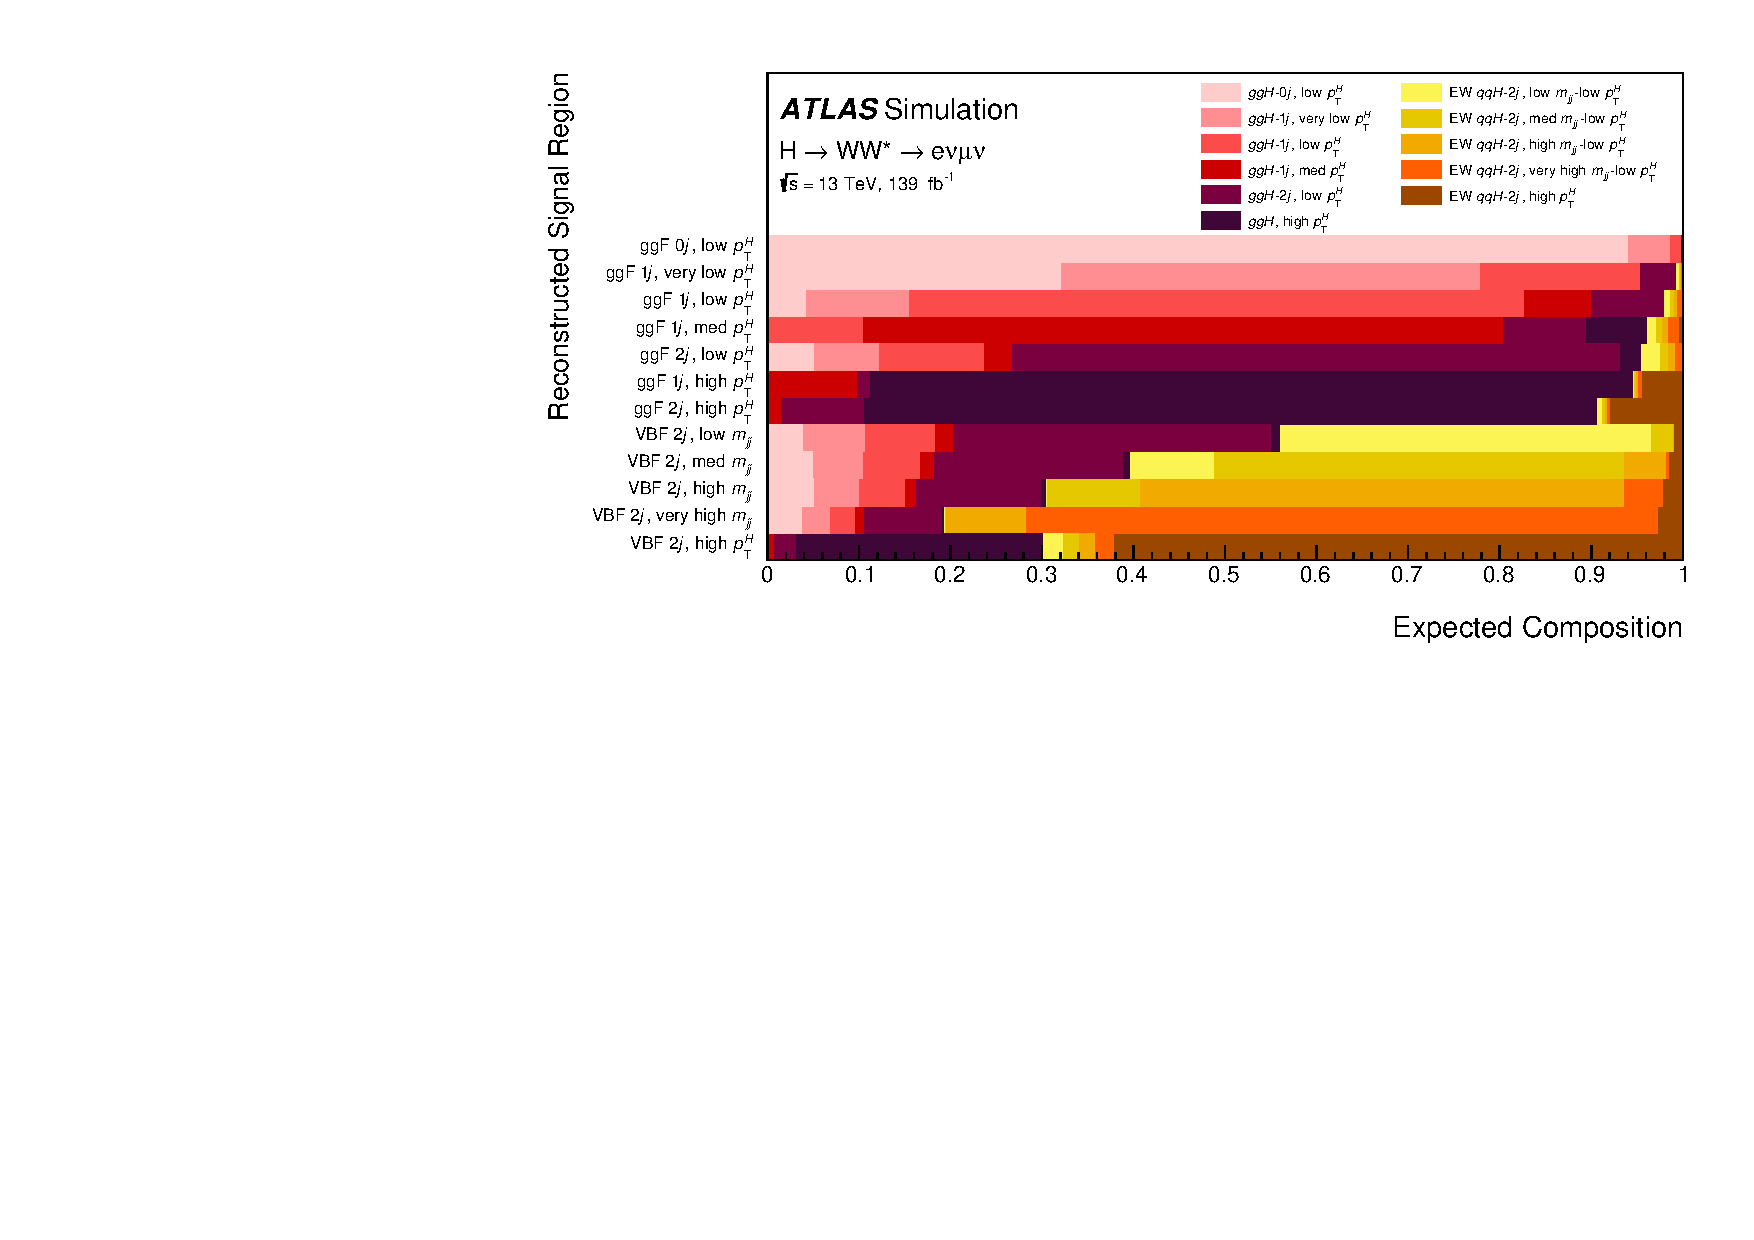
\includegraphics[width=1\textwidth]{\paperfiguredir/11-POI/STXS_CompositionMap}
  \caption{
    Relative SM signal composition in terms of the measured STXS bin for each reconstructed signal region. Taken from \cref{HWWPaper}. 
    \label{fig:STXS_Composition}
  }
\end{figure}
